\section{Path tracing and numerical stability issues}
\label{section:numerical}

\subsection{Description of the problem an heuristic derivation}
Unbiased nature of the brute force volumetric path tracing estimator and physically based
parametrization makes it a perfect candidate for implementing the reference integrator.
The inherent characteristic of the brute force volumetric path tracing estimator is a high variance,
which leads to long rendering times in practice. Being applicable in practice, variance reduction
techniques usually employed. For example Russian Roulette is one of them. The theoretical
description of the Russian Roulette technique can be found in the section \ref{subsection:rr}.

There are different approaches to find the optimal strategy for choosing the Russian Roulette path
termination probability $q_{rr}$ \cite{Veach:1998:RMC:927297}, \cite{And_findinggood}. It is usually
considered as a complicated task, highly dependent on the scene configuration and lighting
distribution. Often the particular value of $q_{rr}$ is based on the local reflectance properties,
accumulated path weight $w_{rr}$ of the material or even exposed to the user as parameter of the
integrator.

The use of Russian Roulette in the context of volumetric path tracing may lead to unexpected loss of
energy during simulations. It is observed as the objects are rendered darker than they should. The
cause of this effect could be the numerical cancellation which appear during rendering of the high
albedo materials with high scattering coefficients. These materials with scattering distance much
smaller than the characteristic object scale $L$ and low attenuation are characterized by high
transmission coefficient $\sigma_t = \sigma_a + \sigma_s$. Tracing the path inside the volume of
such object requires a large number of random walk steps. 

If $q_{rr}$ is the probability of the path to terminate at each step of random walk, then the
probability of the scattering to continue is defined by $p_{rr} = 1 - q_{rr}$. In case if the
termination is not happening at the current step, the path weight $w_{rr}$ is multiplied by the
$1/(p_rr)$. And after $n$ iterations the weight is equal to:
\begin{equation}
w_{rr} = p_{rr}^{-n}
\end{equation}

As $p_{rr}$ is is a probability and is in a range of $[0,1]$, the value of $w_{rr}$ for large $n$
can lower down to floating point precision.

It is possible to build heuristic approach to estimate the minimum allowed Russian Roulette
threshold parameter on the basis of the scattering properties of the media, while still being sure
that there is no energy is lost because of numerical cancellation.

Let us consider the common case of the rendering scenario when the final pixel values of the
simulation are \emph{in the order} of the 1.0. This is a fair assumption because even the special
cases of rendering images with high dynamic range rarely goes above the values in the order of 100.0
which does not change the conclusions of this section.

Following the basics of the the diffusion theory and the theory of the random walks in 3d
\cite{PRE:8383976}, the expected distance at which particle could be found after $n$ steps of random
walk with the constant step size of $d$ is in the order of $R\sim\sqrt{nd}$. Let us consider the the
geometric object with the characteristic depth $L$. The length of the random walk step of path
tracing is in the order of mean free path scattering length $1/(\sigma_s+\sigma_a)=1/\sigma_t$. We
can expect the particle starting the random walk in this object will leave it, in average, after $n$
steps:
\begin{equation}
n\sim\sigma_tL^2
\end{equation}

As we want to make sure that $w_{rr}$ is not going down to less than the cancellation limit of
$\epsilon\sim10^{-7}$ for the addition of the single precision floating point numbers with
characteristic values in the accumulation buffer $C_0\sim1$:
\[
w_{rr} = p_{rr}^{-n} \sim p_{rr}^{-\sigma_tL^2} > 10^{-7}
\]

\begin{equation}
\label{eq:rr_heuristic}
p_{rr} > 10^{\frac{-7}{\sigma_tL^2}}
\end{equation}

\begin{figure}[h]
    \centering
    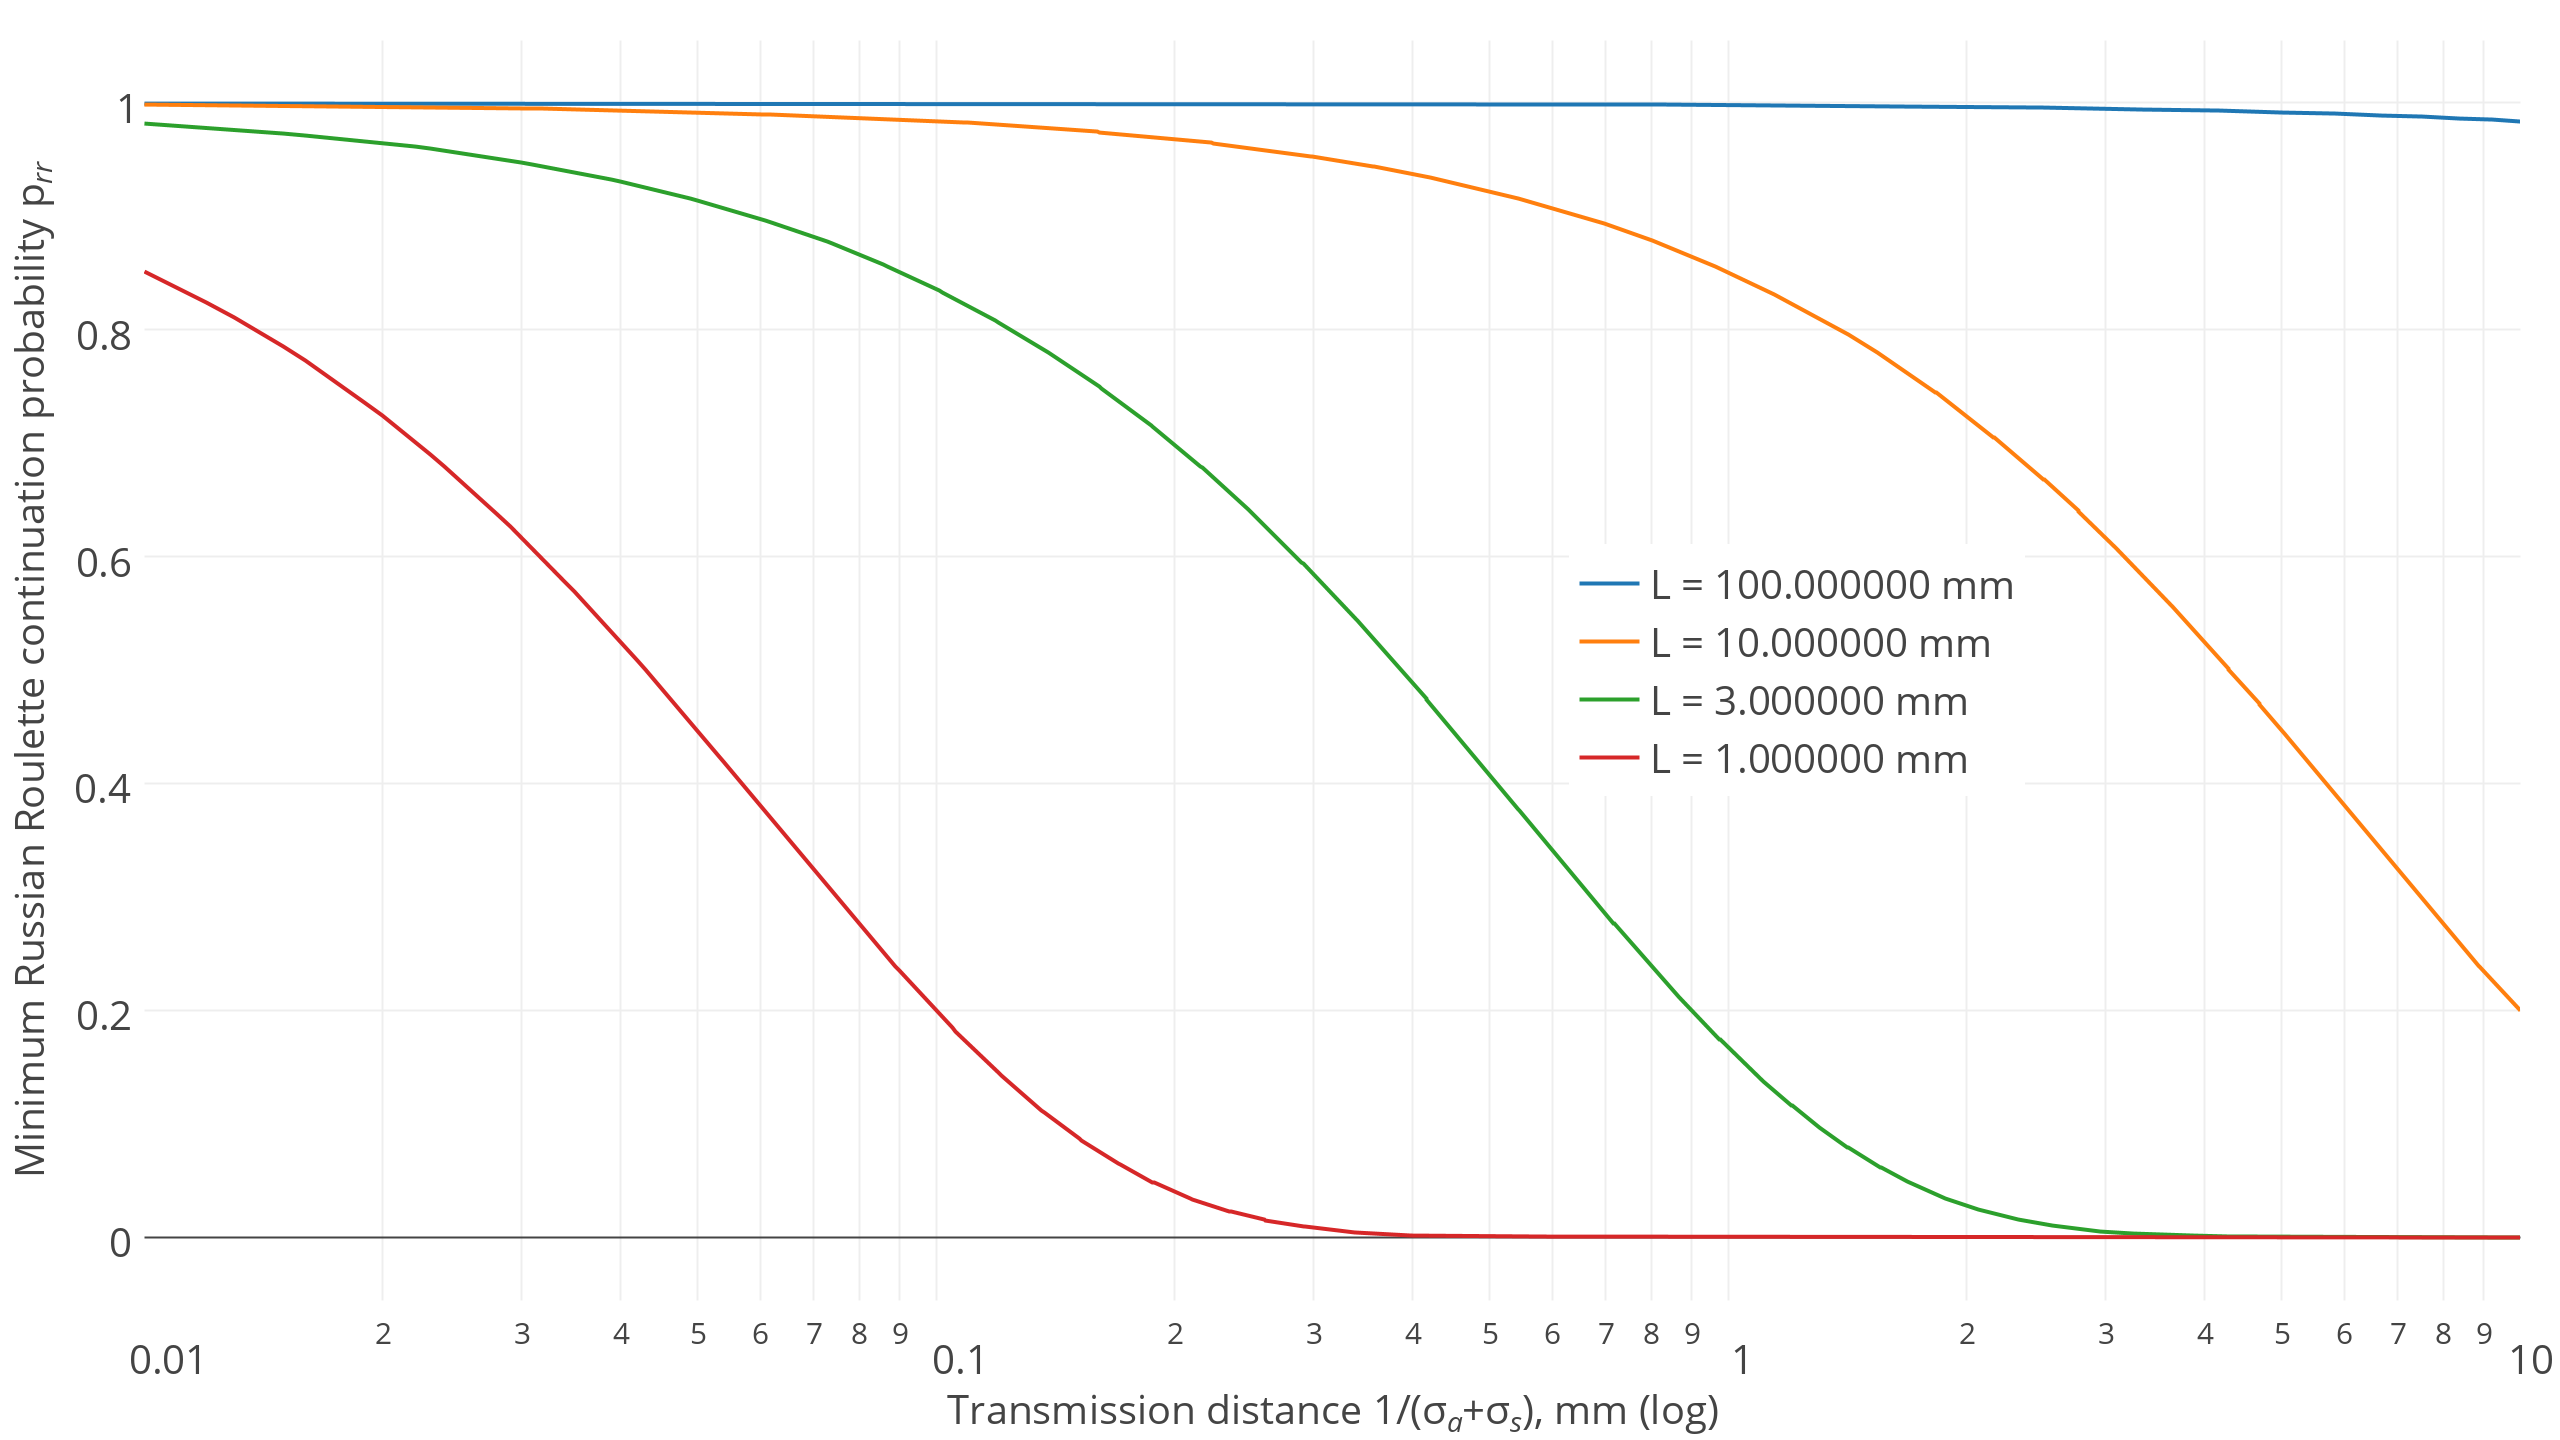
\includegraphics[width=\textwidth]{imgs/plots/rr_heuristic}
    \caption{Minimum allowed Russian Roulette threshold parameter according to heuristic
    \ref{eq:rr_heuristic} for several characteristic object scales}
    \label{fig:rr_heuristic}
\end{figure}

\subsection{Validation of the heuristic}
Simple Furnace test helps us to validate such approximative approach to derive the heuristic
\ref{eq:rr_heuristic}.

In this test we render a cube with length of each side $L=10$mm in 1.0 white environment light scene.
The volumetric albedo of the material is set to 1.0. So that transmission coefficient is defined
only by scattering coefficient $\sigma_a=0.0, \sigma_t=\sigma_s$. This means that all the light
entering the object volume have, in theory, after certain number of scattering events, leave it.
Each pixel of the rendered surface of this cube have to be 1.0 white under such lighting conditions.

We render this cube many times with different values of the scattering coefficient $\sigma_s$ and
Russian Roulette probability $p_{rr}$. You can see the plot of the errors together with the
predicted minimum value of $p_{rr}$ for this object on the figure \ref{fig:rr_heuristic_heatmap}.
\begin{figure}[h]
    \centering
    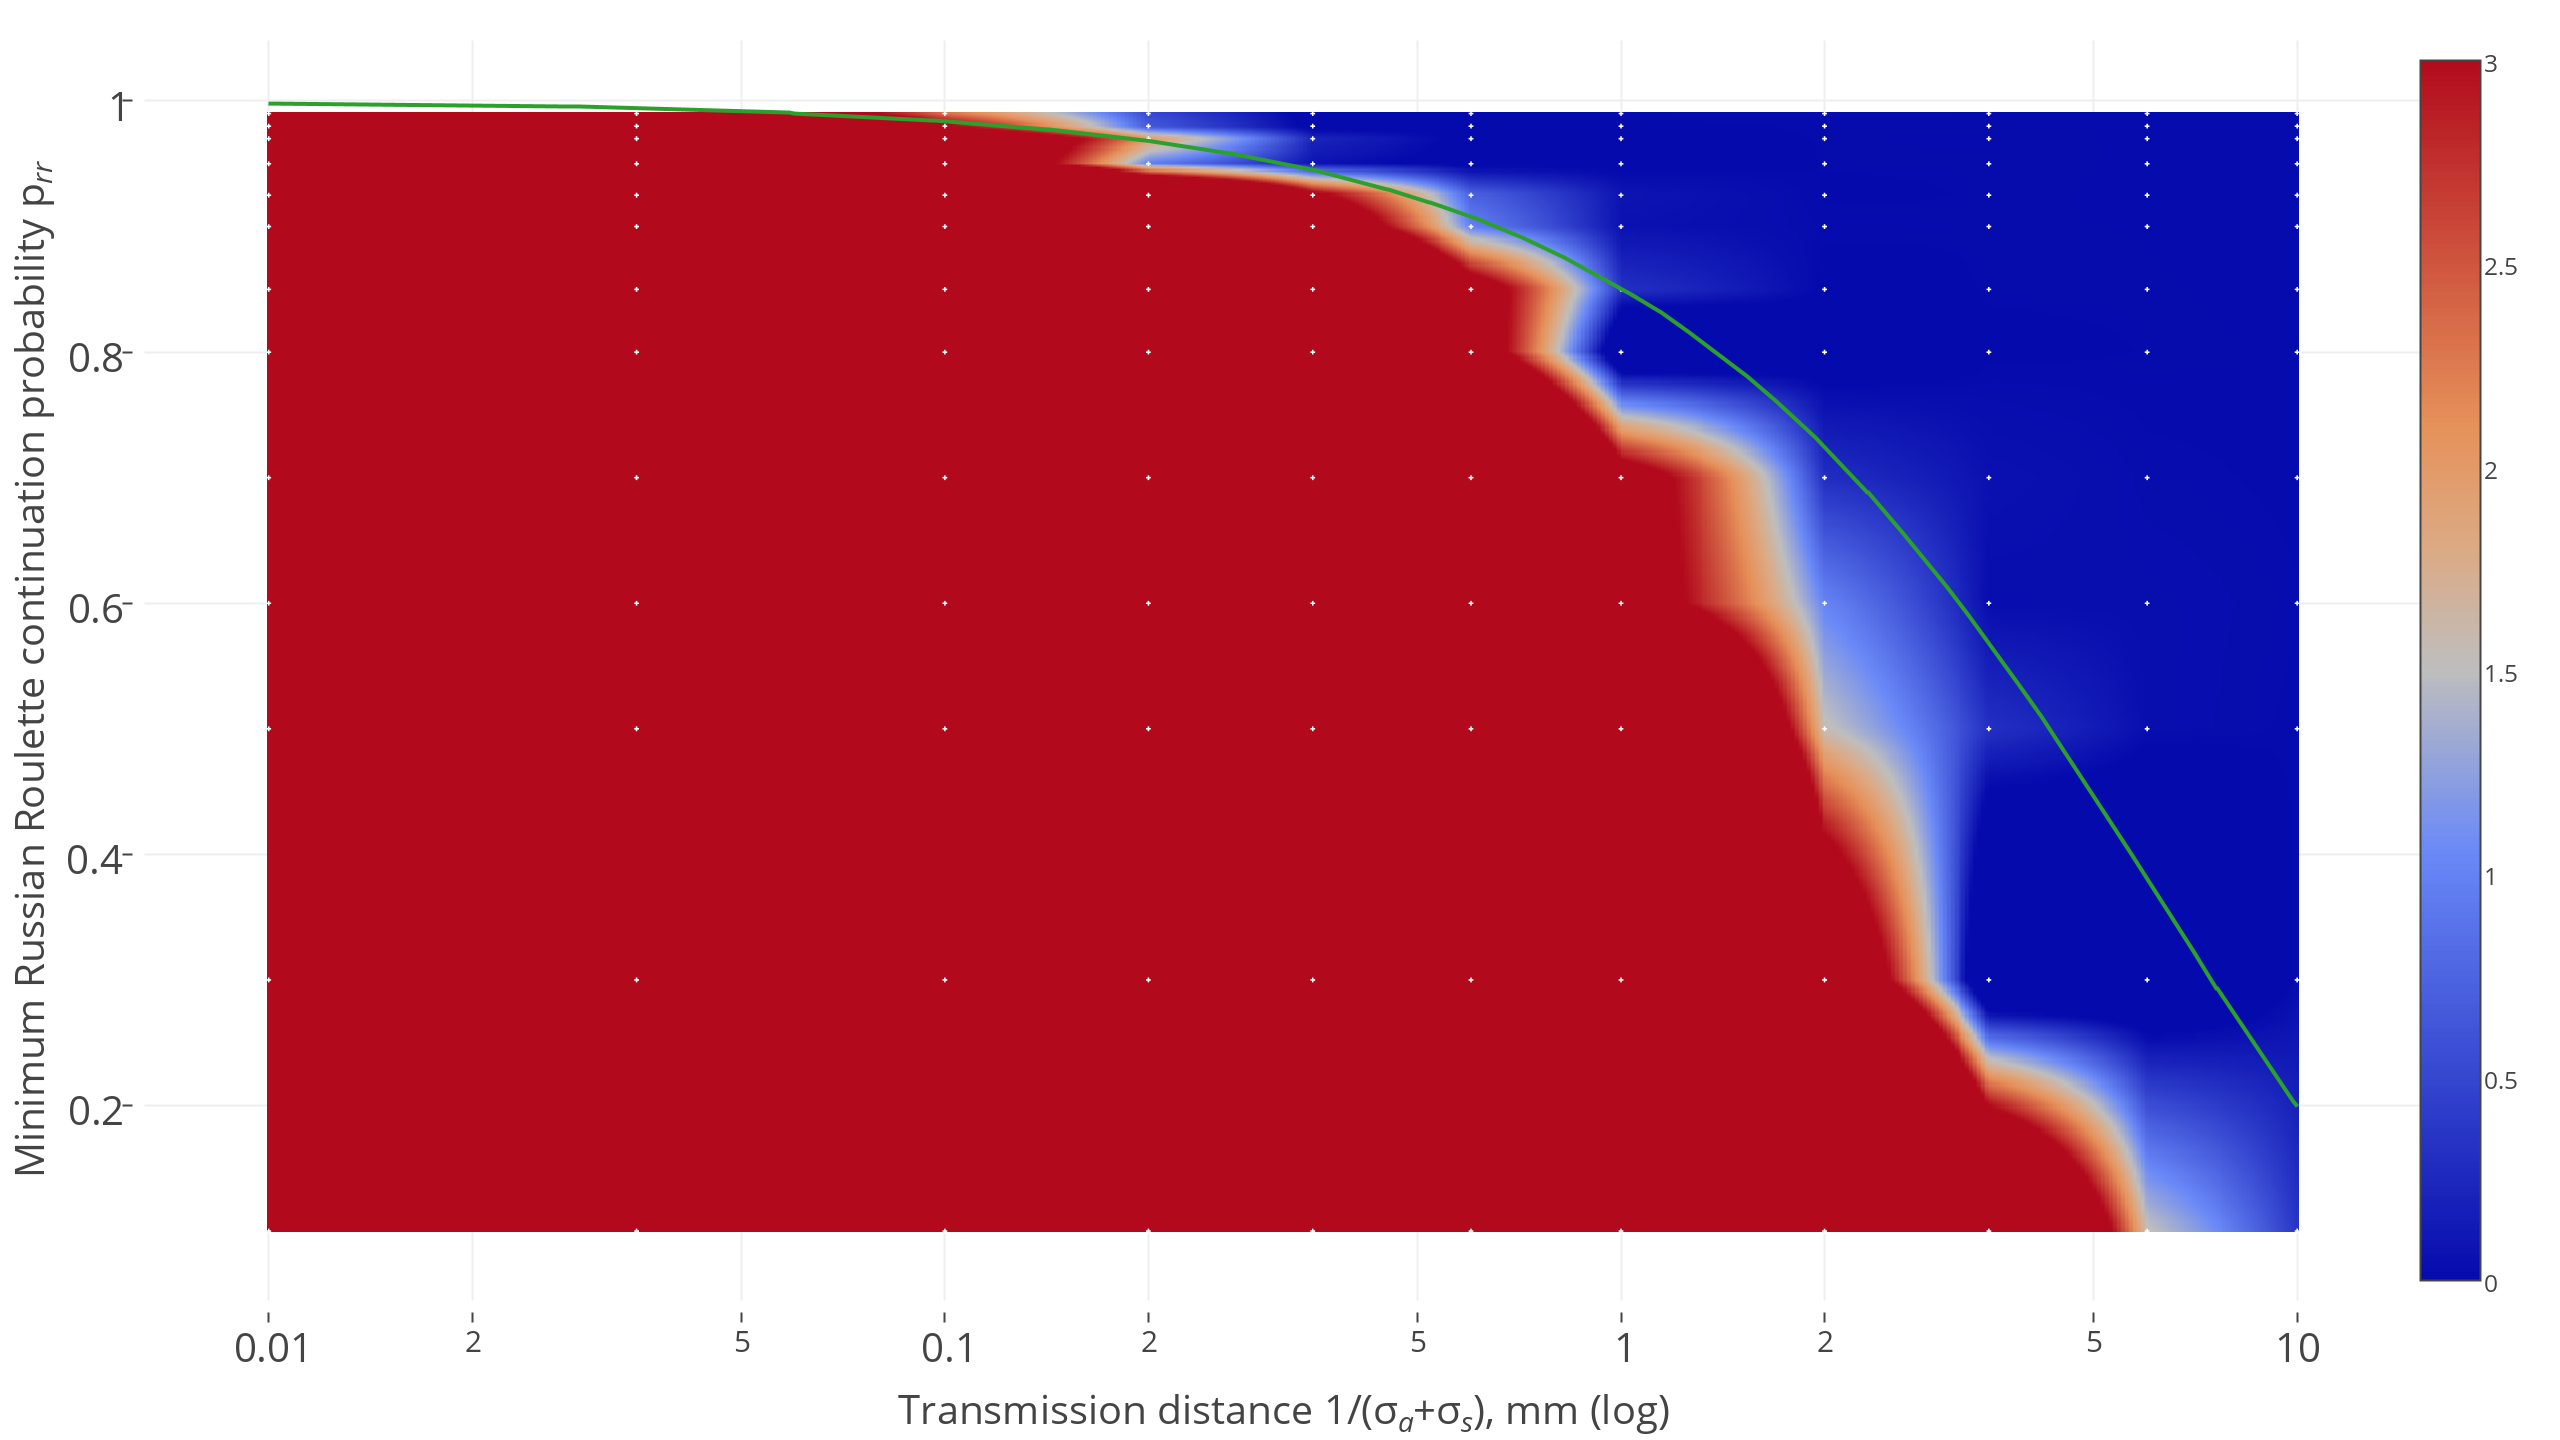
\includegraphics[width=\textwidth]{imgs/plots/rr_heuristic_heatmap}
    \caption{Color coded error of the furnace test with the minimum allowed Russian Roulette
    threshold parameter for L=10mm}
    \label{fig:rr_heuristic_heatmap}
\end{figure}

As seen from the graph, the heuristic gives a good prediction for the lower limit of the  Russian
Roulette continuation probability. In most of the cases where the $p_{rr}$ was set lower than
predicted limit the object was rendered with the loss of energy more than 1\%.

Even taking into account that the heuristic \ref{eq:rr_heuristic} gives a good starting point for
choosing the value $p_{rr}$, it is important to note that the special restrictions on the concrete
application accuracy standards have to be considered. For example, in case of using path
tracing integrator in this thesis as a reference implementation, the Russian Roulette variance
reduction technique was disabled to eliminate any possible numerical issues.


